\documentclass{article}
\usepackage[left=1.9cm, right=1.9cm, top=2cm, bottom=2.5cm]{geometry}
\usepackage{multicol}
\usepackage{enumerate}
\usepackage{tikz}
\usepackage{graphicx}
\usepackage{ragged2e}
\title{\textbf{Extending the BDI Model with Q-learning in Uncertain
Environment}}
\date{}
\begin{document}
\maketitle
\centering
\begin{multicols}{3}
\textbf{Qian Wan†} \\
  Hubei Province Key Laboratory of Intelligent Robot\\
  School of Computer Science and Engineering, Wuhan Institute of Technology\\
  Wuhan, China
\vfill\columnbreak

\textbf{Wei Liu} \\
  Hubei Province Key Laboratory of Intelligent Robot\\
  School of Computer Science and Engineering, Wuhan Institute of Technology\\
  Wuhan, China
\vfill\columnbreak

\textbf{Longlong Xu} \\
  Hubei Province Key Laboratory of Intelligent Robot\\
  School of Computer Science and Engineering, Wuhan Institute of Technology\\
  Wuhan, China

\end{multicols}
\justify

\begin{multicols}{2}
\section*{ABSTRACT}
The BDI model has solved the problem of reasoning and decisionmaking of agents in a particular environment by procedure
reasoning. But in uncertain environment which the context is
unknown the BDI model is not applicable, because in BDI model
the context must be matched in plan library. To address this issue,
in this paper we propose a method extending the BDI model with
Q-learning which is one algorithm of reinforcement learning, and
make an improvement to the decision-making mechanism on the
ASL as a implement model of BDI. Finally we completed the
simulation of maze on Jason simulation platform to verify the
feasibility of the method.
\section*{KEYWORDS}
BDI model, Agent, Q-learning, Jason, Plan Library\\
\textbf{ACM Reference format:}
Qian Wan, Wei Liu, Longlong Xu and Jingzhi Guo. 2018. Extending the
BDI Model with Q-learning in Uncertain Environment. In Proceedings of
2018 International Conference on Algorithms, Computing and Artificial
Intelligence (ACAI’18). Sanya, China, 6 pages.
†Corresponding author: 1007831839@qq.com
Permission to make digital or hard copies of all or part of this work for personal or
classroom use is granted without fee provided that copies are not made or


\section{Introduction}
The research on agents, acting in an uncertain and dynamic
environment is a challenge, BD I [1] agents is designed for agentorient programming model and build multi-agent systems. BDI
model is concerned with agent’s rule description and logic
reasoning in multi-agent systems. However these two factors are
based on context and must be designed in advance.
Reinforcement learning [2] (RL) is applied to solve this problem
that BDI agent don’t know environmental model. RL assumes
that an agent is using observed rewards that are perceived from
the environment to measure its utility following its actions in an
uncertain and dynamic environment. According to reward value,
the agent can determine the sequence of actions though in
uncertain environment.
BDI concepts used to describe people's behavior and intention
at first, then was introduced into artificial intelligence, and the
earliest BDI abstract model was put forward by Georgeff. On
the basis of the model, different Procedure Reasoning System
(PRS) are designed for reasoning. Based on PRS mode, the
researchers developed the Multi-Agent System (MAS) based on
BDI model including JACK [3], DECAF [4], IRMA [5],
JADEX [6],ASL [7], etc. Because the ASL which has been
added with the plan library on the foundation model of BDI has
a simulation system and a better extension interface, we see
ASL as a starting point for studying the BDI model. The plan
problem of the agent in uncertain environment, so our research
is aimed at improving the planning part of the ASL which is the
implementation model of the BDI Agent.
RL is learning to map situations to actions so as to maximize
a numerical reward. Without knowing which actions to take, the
learner must discover which actions yield the most reward by
trying them. Actions may affect not only the immediate reward
but also the next situation and all subsequent rewards. Agent in
RL has the ability of learning and planning, but lacks the logic
and reasoning ability of BDI Agent.RL can be divided into two
types by the: model-based and model-free, model-free RL is
mainly used to solve the planning of agents in situations where
environmental information is not known, Q-learning is one of
non-model algorithm that has high learning efficiency.
Therefore, this study put forward the method which can solve the
problem that BDI Agent can't decision under dynamic and
uncertain environment by RL.
The structure of this paper is as follows. After this introductory
section, we follow in Section II with a brief discussion of related
works. Section III introduces BDI Agent and AgentSpeak(L), RL
and q-learning algorithm. Section IV describes our method that
decision improvement algorithm based on q-learning in ASL
system. Section V describes the simulation experiment and
evaluates and analyzes the results of experiment. Section VI
summarizes our research and point to possible future developments.

\section{Related Works}
The inference mechanism in BDI model is based on the preset
environment, so the BDI system lacks the planning under
unknown environment. For the known environment model, there
have been many methods are used to solve the planning in which
including decision tree, self-aware neural network, and rules
learning algorithm are used to optimize the Agent’s decision.
Pereira apply Markov decision process to generate the optimal
strategy of BDI plan, but the method in unknown environments is
difficult to build Markov environment model, so these methods do
not apply in unknown environment information.
For the unknown environment model, the self-adaptive research
of agent in the unknown environment of BDI model has been paid
more attention. Google recently proposed a method that building
the BDI model of Agent by deep reinforcement learning to
understand the current real intention of Agent in order to improve
its planning [8], J. L. Feliu propose to have an offline training
session for plan generation in an uncertain and dynamic
environment, the use of Q-learning from training sessions
consisting of interactions between agent and environment
generates plans for agents in ASL[9]. Although this method has
solved the problem that agents know how to act when considering
the efficiency of achieving goals in every state under uncertain
environment, but when the state set is too large, quantity of
generated plan will be explosive which lead to deviation that
agents focus on the internal logic in original BDI model. Joost
Broekens propose to solve the problem for selection of rules of
which priority is learned by RL, and to use a state to represent
independent heuristic rules on active targets [10]. However, it is
difficult for agents to express the state in dynamic environment.
Autonomous Agent mentioned in the literature [11], incentive
signal of agent's behavior is given by the person. Supervised
learning is used to generate action selector according to the
excitation signal which finally enables the agent to perform the
task efficiently in complex and unknown environment, this
method enables the Agent to learn the human’s perception and 
decision. But the human resource is consumed by the human
being as the trainer.
Compared with the above method, this study avoids the unit of
plan with the state as the plan and the decision- making in the
unknown environment will become a plan which added to the
plan library after the Q-learning algorithm has explored the
environment. The plan is the unit after learning which avoids the
problem of oversize planning library, and the state of agent is
easy to define.
\section{Background}
\subsection{ BDI-Agent and AgentSpeak(L)}
Programming paradigm based on agent gives higher intelligent
computer software module and adaptive ability, BDI is an agent
oriented programming model which is composed of Belief, Desire
and Intention. The belief includes the environmental information
acquired by the agent from the environment, the information of its
own operation and the information received from other agents.
The desire represents the possible state of the agent when
performing task, which is driven by intention in the actual
operation. The intention represents the state that the agent decides
to achieve in the actual operation of the agent. There are two types
of intention one of which is the target to be executed by the agent,
and another is the plan based on the context matching in the BDI
model. The BDI conceptual model is described as follows: agent
initializes beliefs and intentions, then perceives environmental
information. By belief update function, belief is update.
According to the current intentions and beliefs, some desires are
selected as a candidate, one of them can be selected as the
execution plan through the matching rules that have been
designed in advance. Agent finish the task by the plan. BDI model
is a conceptual model in which the agent has basic logical
reasoning ability.
ASL (Agent Speak Language)[12] is extended on the basis of
BDI model, and the specific system structure diagram is shown
in figure 1.
\begin{enumerate}[1.]
    \item The agent target and belief library are initialized, the belief
library is updated by the BRF (Belief Revision Function)
according to the target agent perceives information from the
environment or from other agents.
    \item The agent cognitive the environment changes, and updates
the belief library and verify whether the change triggers the
event in the plan library. When multiple events are triggered
simultaneously, the sequence of event execution is
determined by the SE function
    \item According to the trigger event, the predicate symbol is
matched in plan library. For example, if default trigger
event in the plan library is +color(Object,color). When
agent perceives the blue box from the environment, the data
will be transformed into expression +color
(box1,blue)[source(percept)], then after SE(Select Event)
is used to match trigger event,box1 Object, blue
Color. The applicable plan will be matched, and the value of Object and Color is instantiated into box1 and blue entities
in the plan.
    \item Select a plan through the $S_0$ function which context is matched in the applicable plan, the plan structure is \textit{trigger event:context -$>$ body, body} content includes the action sequence, subtarget and child trigger event.

    \item According to the context, such as \textit{boxl $=1 \mathrm{~m}^2$}, context expression\textit{ Object $>0.5 \mathrm{~m}^2$}, and there may be subgoal which is matched similarly in body. The plans that conform to context are pushed into the stack of intent. The agent performs the action in turn to pop up the stack. When the stack is empty, the system enters the next loop.
\end{enumerate}
AgentSpeak(L) builds a multi-agent system based on BDI
model, which facilitates the programming and research of Agent.
This study mainly focuses on the improvement of ASL which is
the implementation model of BDI.

\subsection{ RL and Q-learning}
Reinforcement learning is completely different from other
machine learning algorithms such as supervised learning and
unsupervised learning. It requires interaction with the
environment and obtains “experience” from the environment.
Most of the reinforcement learning adopts Markov model of
which the most important feature is that the next step in the
current state is not relevant to the past, RL can be described in the
Markov decision process. The definition of Markov decision
process is as follow \textit{$M=(S, A, P, r, \gamma, N)$  S}
is the state set of
agent. \textit{A} denotes the action set of agent. P
represents the transfer
probability between states, r is the immediate reward of a state
transition $\gamma \in [0,1]$
is a discount factor, N is the number of steps
from the initial state to the final state. The cumulative reward
denote with $R=\sum_{n=0}^N \gamma^t r_t$ The goal of reinforcement learning is to find
the optimal strategy to maximize the cumulative reward of a state transition value of
the function which denote with $\max _\pi \int R(\tau) P_\pi(\tau) d \tau, \tau$ represents the
behavior trajectory of the agents $\tau=\left(\mathrm{s}_0, \mathrm{a}_0, \mathrm{~s}_1, \mathrm{a}_1, \ldots ..\right)$
Q-learning algorithm which is one of the RL is mainly used for
agent decision learning under the model in which agent does not
know the information of environment. Q-learning utilize the statebehavior function Q(s,a) to indicate the cumulative reward of the
new state to the final state when the state s performs action a, and the maximum value of Q(s,a) is updated every time the state is
passed. Its iterative update equation is given in equation (1):\\
$\mathrm{Q}_{\mathrm{k}+1}\left(S_t, a_t\right)=\mathrm{Q}_{\mathrm{k}}\left(S_t, a_t\right)+\alpha\left(\mathrm{r}_{t+1}+\gamma \max _a \mathrm{Q}_k\left(S_{t+1}, a\right)-\mathrm{Q}_k\left(\mathbf{S}_{\mathrm{t}}, a_t\right)\right)$ \\

$\mathrm{Q}_{\mathrm{k}+1}\left(S_t, a_t\right)$ represents the value of the updated cumulative reward
obtained by performing the action at time t. $\mathrm{Q}_{\mathrm{k}}\left(S_t, a_t\right)$
represents
the cumulative value of the last time the Agent passed the state.
$\alpha \in(0,1)$, the larger $\alpha$ is, the later reward is more considered. $\mathrm{r}_{t+1}$ represents the value of the reward obtained when $S_t$ performs action a to $S t+1 . \gamma$ is the discount cumulative reward. $\max _a \mathrm{Q}_k(s t+1, a)$ denotes the maximum value at $S_{t+1}$ in Q table. Q-  learning is a greedy strategy algorithm. The value of Q(s, a) tends
to be stable after the finite iteration of formula (1), the maximum
current state Q value in the Q table is selected until the final state
is reached to form the optimal strategy.

\begin{figure}[h]
\centering
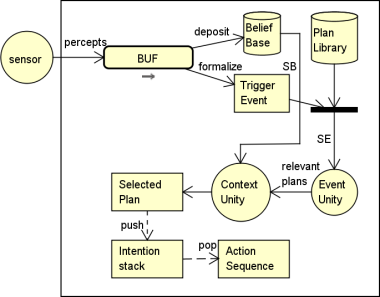
\includegraphics[width=0.3\textwidth]{fig1.png}
\caption{ASL Arquitecture}
\label{figura1}
\end{figure}


\section{The ASL Optimal Decision Algorithm Based On
Q-learning}
he ASL reasoning model is shown in figure 1. The context of an
agent consists of trigger events and environmental information.
But in an uncertain environment, there be no plan for matching
context, another problem is that agent need to consider which plan
is the best when multiple contexts are matched in plan library. In
view of the above problems, this paper proposes an ASL optimal
decision algorithm based on q-learning by which BDI agent
improve the plan library in ASL. This study mainly improves the
planning library from two aspects. (i) For multiple plan decision
problems, the task is completed at each times, the cumulative
reward value is recorded and compared with the latest plan.
Choose the plan with the largest cumulative reward as the next
execution plan. (ii) In the uncertain environment, agents explore
the environment and accept the feedback of the environment. By
using q-learning algorithm training, the best sequence of actions is
completed and the plan is added to the plan library.
The detailed algorithm of ASL optimal decision improvement
algorithm improvement details are shown in figure 2. In the initial
environment model, because RL is based on markov decision
model,you need to define the state s that the agent may exist, the
corresponding reward value \textit{r}, the plan library \textit{Pu} and trigger
event \textit{E}.\\
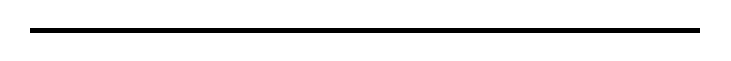
\begin{tikzpicture}
  \draw[line width=2pt, color=black] (0,0) -- (8.5,0);
\end{tikzpicture}
ASL optimal decision algorithm based on q-learning:\\
\begin{tikzpicture}
  \draw[line width=0.5pt, color=black] (0,0) -- (8.5,0);
\end{tikzpicture} \\
Input: $\mathrm{E} \quad / * \mathrm{E}$ are initial trigger event$* /$ \\
$\mathrm{P} \quad / * \mathrm{Pu}$ are initial plans in library */ \\
$\mathrm{Su}, \mathrm{rt} / * \mathrm{Su}$ is set of states, rt are reward */\\
output: $\pi \quad / * \pi$ is the agent's strategy $* /$\\
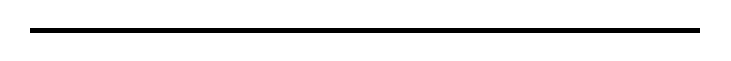
\begin{tikzpicture}
  \draw[line width=2pt, color=black] (0,0) -- (8.5,0);
\end{tikzpicture}\\
1: if match(E,P) \\
2:$\mathrm{N}++; / *$ calculate number of matched plan */ \\
3:if $(\mathrm{N}==1)$ 
\end{multicols}
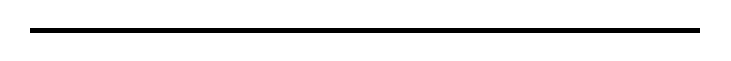
\begin{tikzpicture}
  \draw[line width=2pt, color=black] (0,0) -- (8.5,0);
\end{tikzpicture}


\end{document}


\end{document}
